\newpage
\chapter{Project Logic Diagrams}
\label{ch-diagrams}

In a large project such as the Design Synthesis Exercise, a planning and task has to be made and followed to keep the design process organised.


\begin{figure}[h]
    \centering
    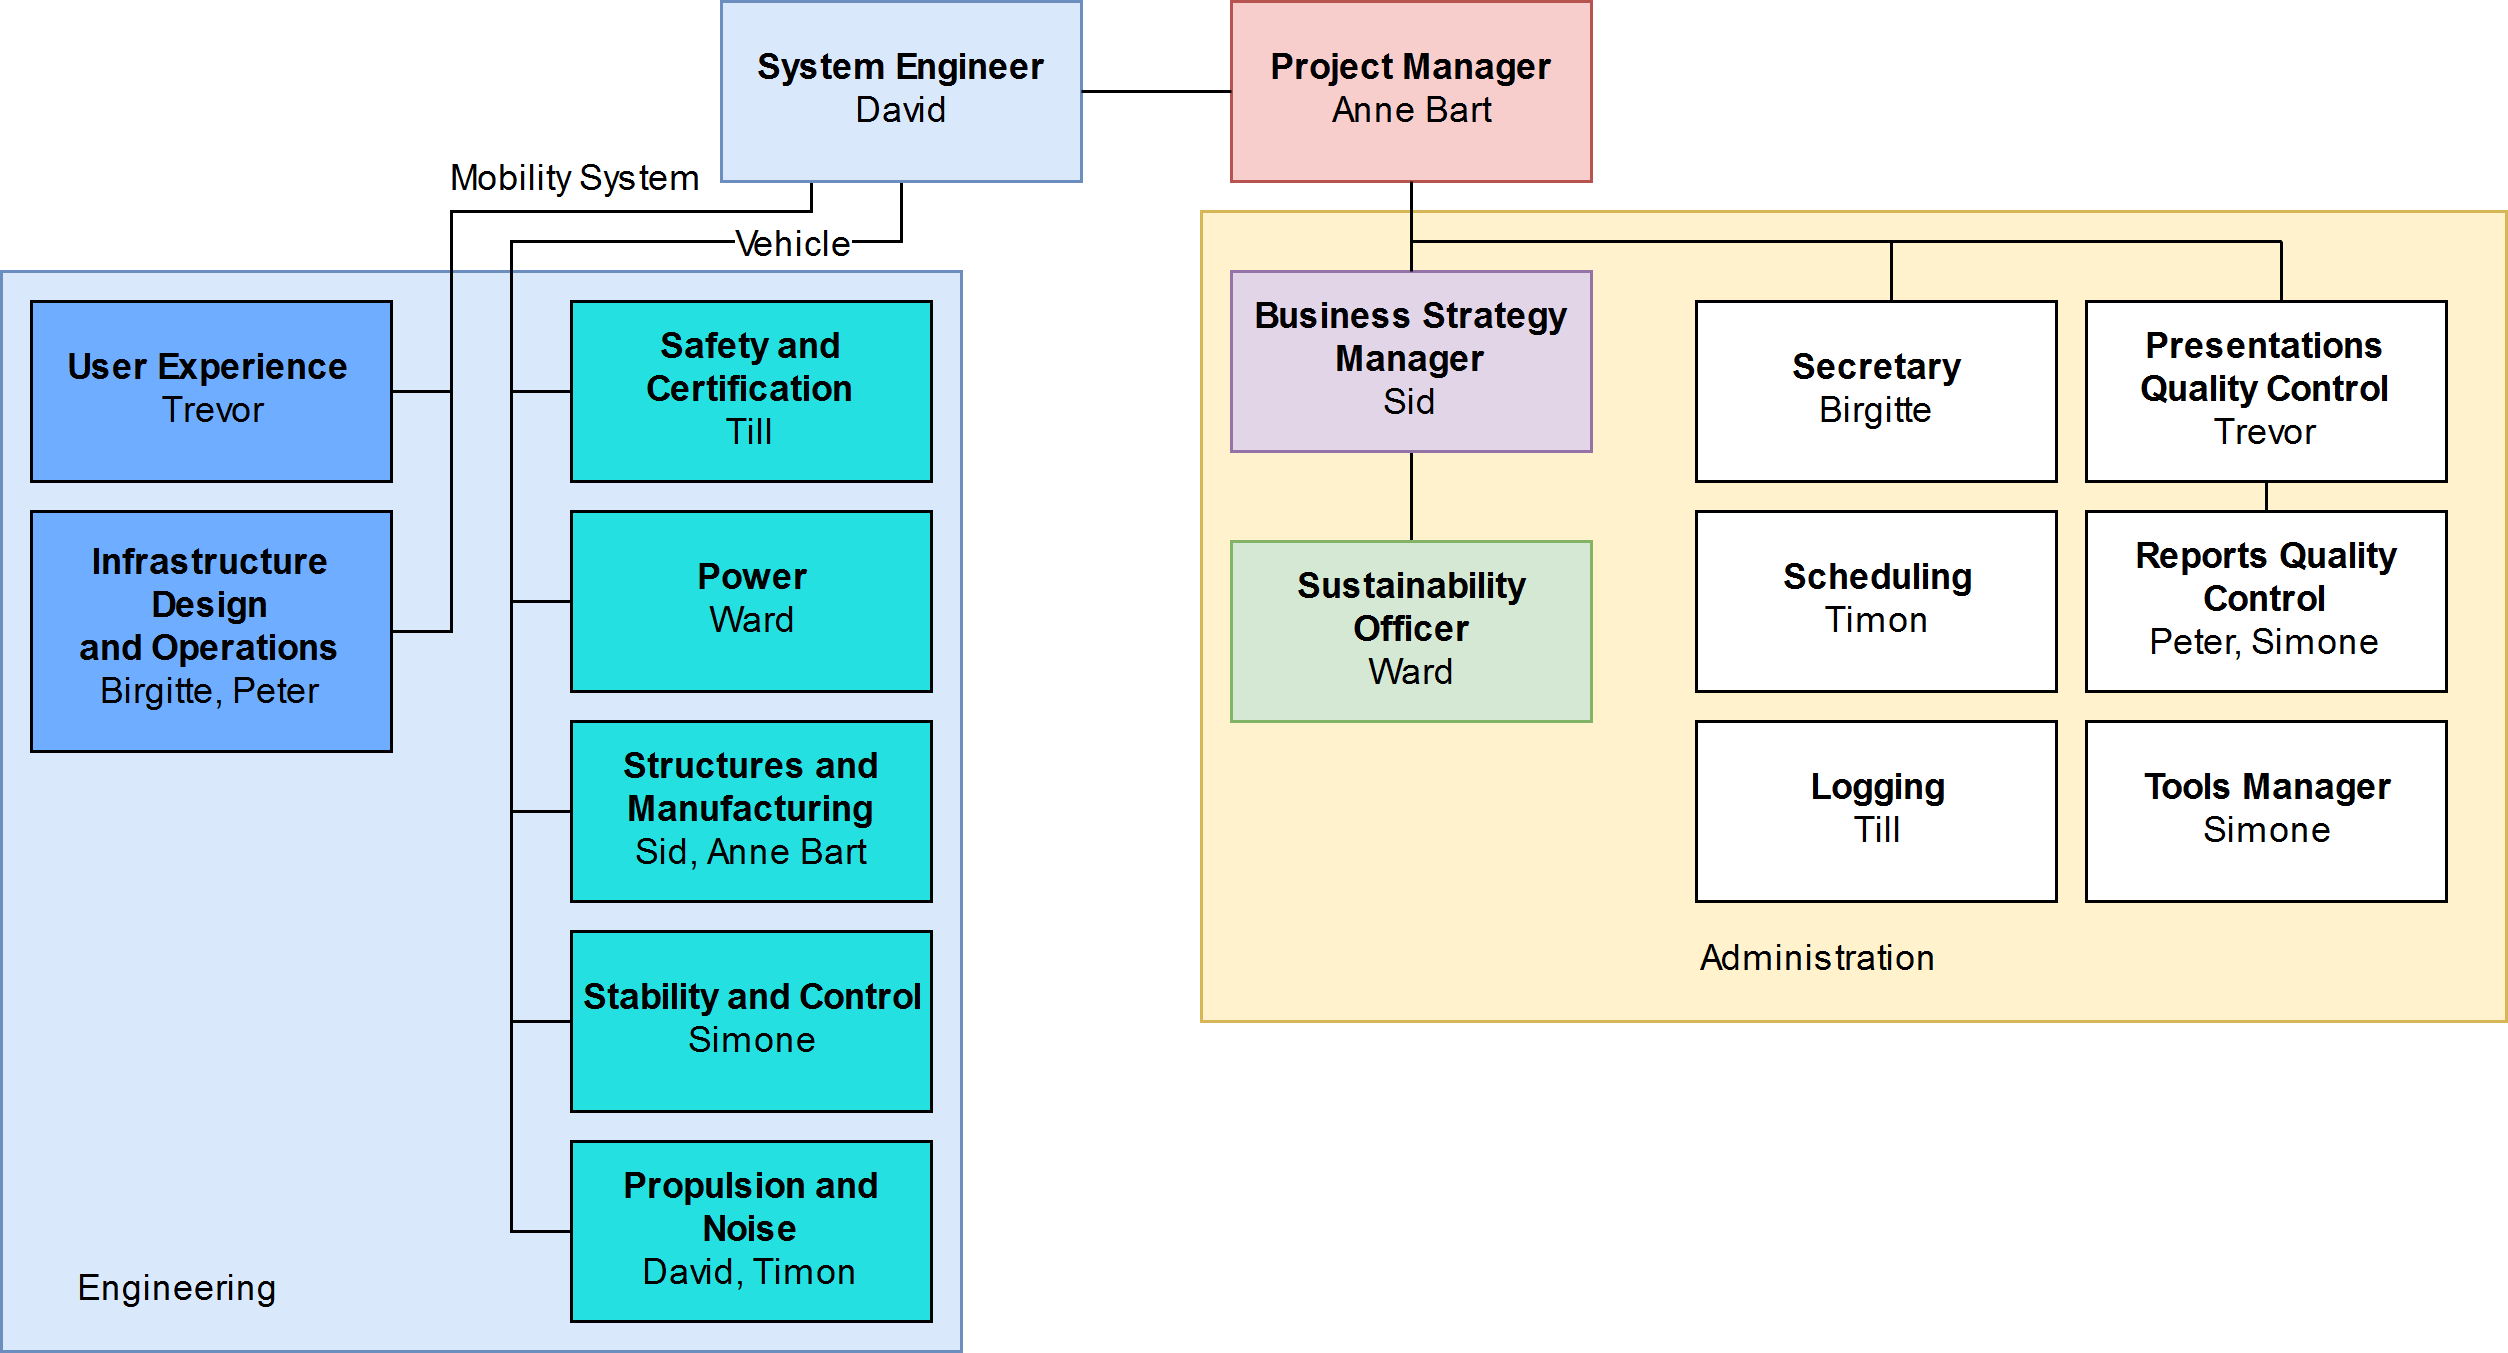
\includegraphics[width=0.9\linewidth]{Figures/organigram.png}
    \caption{Team organigram}
    \label{fig:organigram}
\end{figure}


The Work Flow Diagram, the Work Breakdown Structure and Gantt Chart are visual tools that can help in project planning, scheduling, HR allocation, and in keeping a clear overview of the sequential and parallel steps that bring the project from its start to its completion. In the included diagrams, all tasks are given identifiers. The first initials indicate the phase, followed by the deliverable number. After the hyphen, Work Packages (WP) are given a number and tasks a letter. Generally a WP should contain 2-7 tasks and each task takes from 1 to 8 hours to complete without interruption. The labelling convention is the following: $\underbrace{\text{BR}}_\text{Phase}\underbrace{01}_\text{Deliverable ID}-\underbrace{02}_\text{WP ID}\underbrace{A}_\text{Task ID}$ 

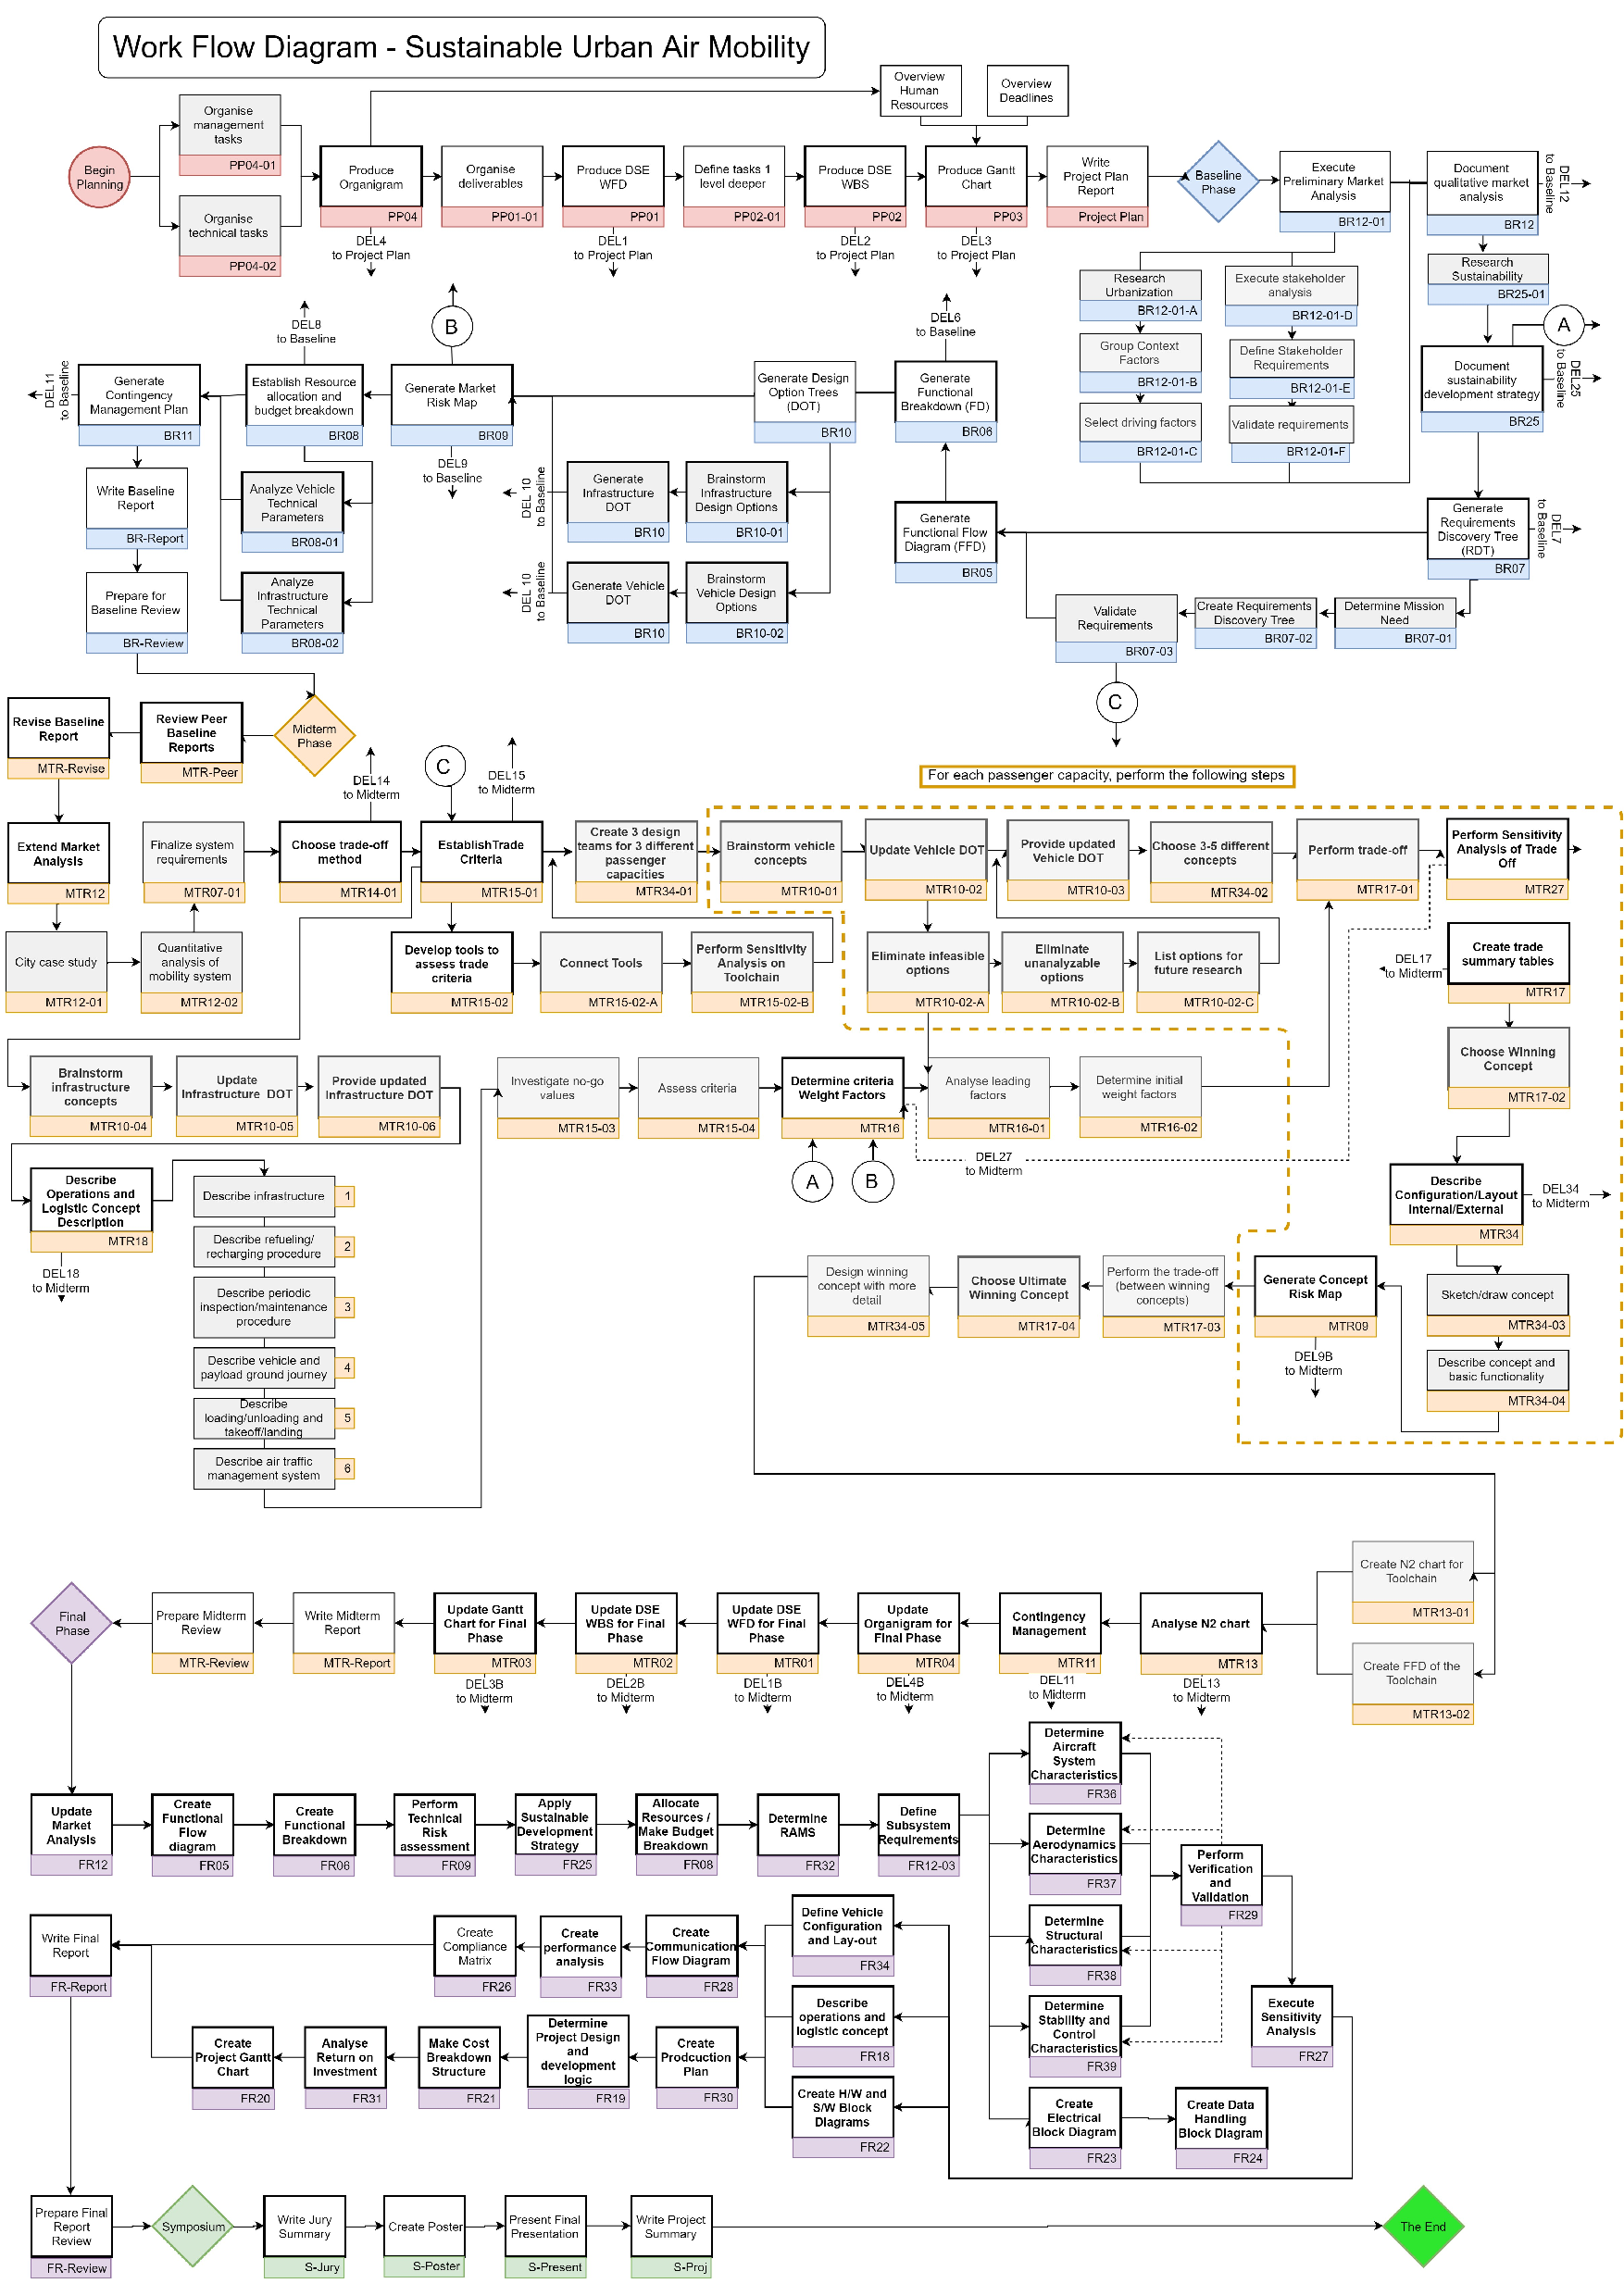
\includepdf[pages={1},fitpaper]{Figures/WFD_MTR.pdf}

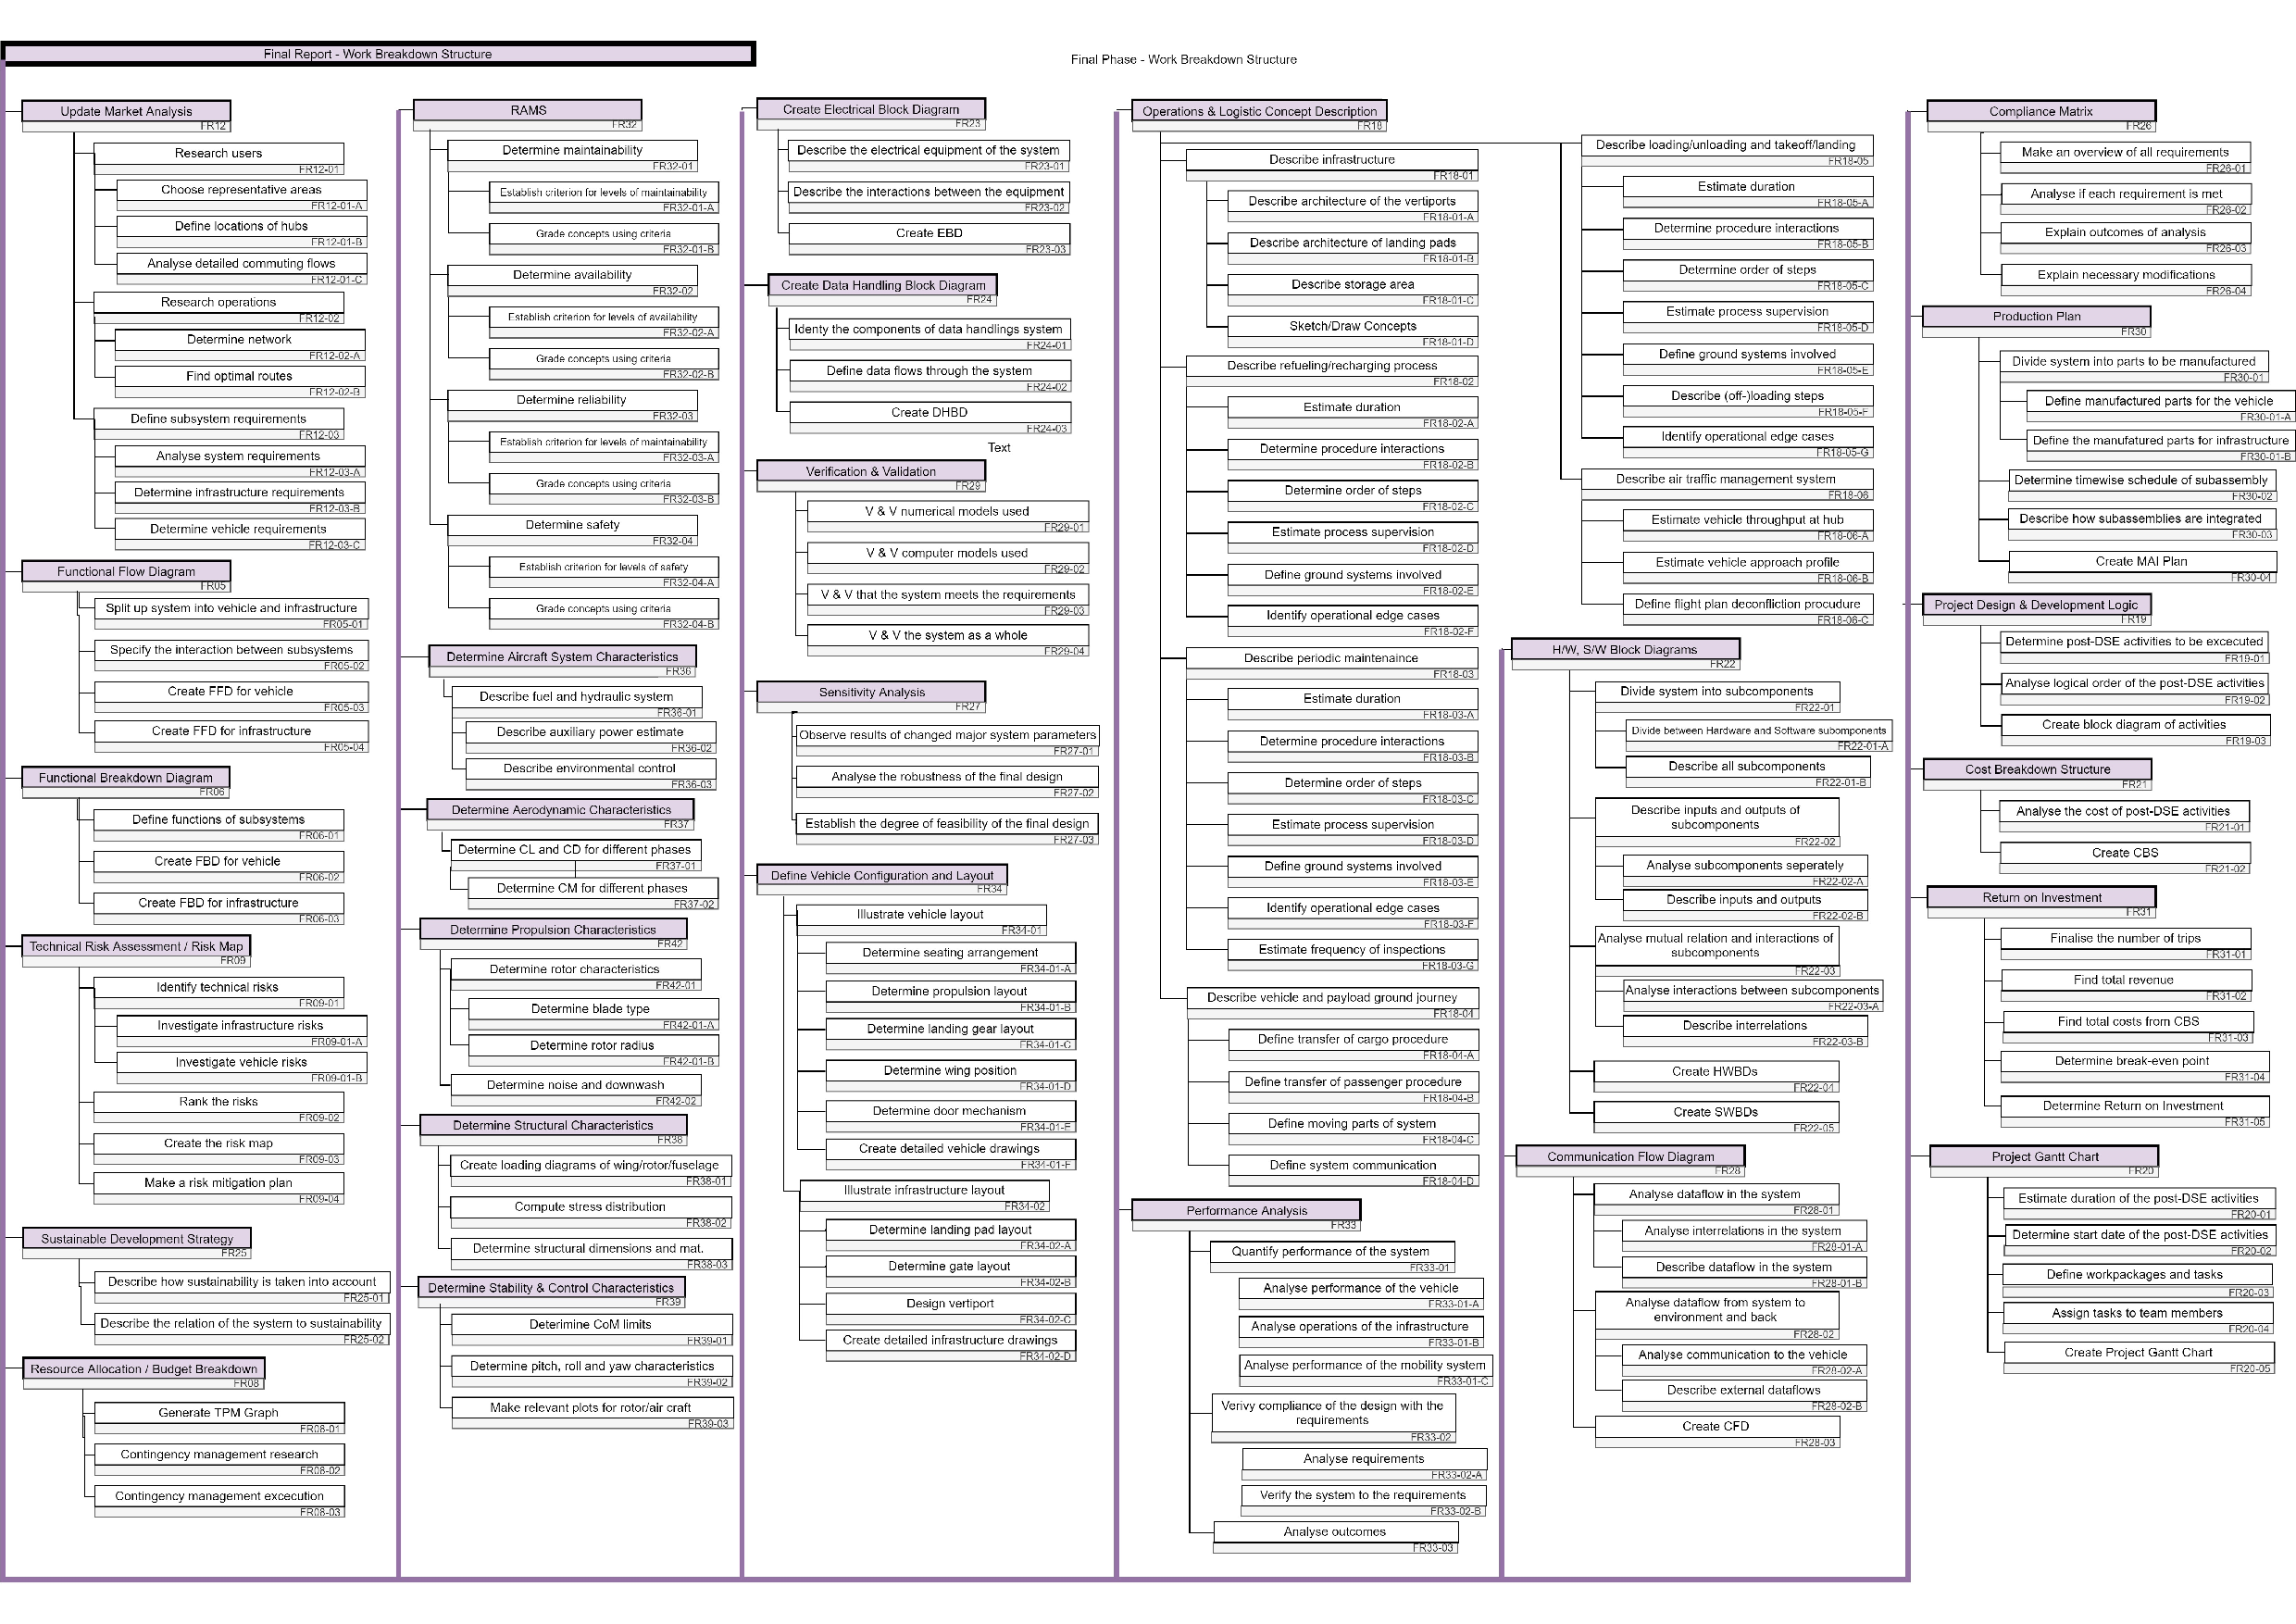
\includepdf[pages={1},fitpaper]{Figures/WBS_MTR.pdf}

